% !TeX spellcheck = en_US
\documentclass[a4paper,titlepage]{article}
\usepackage[margin=1.25in]{geometry}
\usepackage{blindtext}
\usepackage{enumitem}
\usepackage{xcolor}
\usepackage{hyperref}
\usepackage{graphicx}
\usepackage{caption}
\usepackage{float}
\usepackage[htt]{hyphenat}
\usepackage{amsmath}

\title{STAD68 Draft: Comparison of Random Forests and Support Vector Machines (SVM)}
\author{Guan Yu Chen\\ 1001591967}
\date{Due: November 23, 2018}
\usepackage{fancyhdr}

\pagestyle{fancy}
\fancyhf{}
\lhead{STAD68}
\chead{Draft}
\rhead{Guan Yu Chen}
\rfoot{Page \thepage}

\begin{document}
	\maketitle
	\section{Introduction}
	There are lots of machine learning algorithms to use on certain datasets and the decision might be difficult on which one that has the better performance and accuracy. Specifically, this report aims to compare the accuracy and performance of Random Forest and Support Vector Machine (SVM). The dataset that will be used for this comparison is a wine dataset. 
	
	Red and white wine are enjoyed by many around the world but some are tastes better than others. The goal is to analyze different quality red wine, in particular the Portuguese "Vinho Verde". The analysis aims to given a set of characteristics of the wine, is it possible to predict the quality as well as given the quality, is it possible to determine the characteristics.
	
	The dataset \footnote{dataset available at \url{https://www.kaggle.com/uciml/red-wine-quality-cortez-et-al-2009}} has a total of 1599 observations, 11 features (not including reponse variable) and 1 response variable. Some of the features in the dataset include fixed acidity, citric acid, pH Scale, Alcohol level, residual sugar.
	\section{Random Forest}
	Random Forest is an ensemble method that can be used for classification and regression. It constructs a multitude of decision trees when training and outputs the class (classification) or mean prediction (regression). Using Random Forests avoids chances of overfitting which single decision trees can do. The implementation of Random Forest is done in Python using built-in libraries. In \texttt{sklearn.ensemble}, which is Sci-Kit Learn library ensemble methods, there is a \texttt{RandomForestClassifier}. To use it, the hyperparameters needs to be adjusted and fit/train the model to the training data. After tuning the hyperparameters, we can test the model on the testing data in order to estimate the true risk. For the metrics, another library was used called \texttt{metrics} from \texttt{sklearn}, this library computes the precision, recall, F1-Score and mean (weighted in some cases) precision. 
	\subsection{Training / Cross Validation}
	In order to have enough data to train the Random Forest model, the designation for training and testing set is 70\% and 30\% respectively. This model will focus on building a model to predict good wines since there is more data available. Random Forest can do cross validation in the algorithm with Out-Of-Bag (Out-Of-Bag error), which uses the samples are not used any decision tree to validate the model. Currently, with 1000 trees, using entropy to determine splits, the Out-Of-Bag Score/Error is 0.904 (90.4\%). 
	\subsection{Testing Data / Risk}
	Having our training model and the hyperparameters tuned, this model is used on the testing set to see its precision and performance. The chart below shows the results from running the model on the testing set.
	\begin{table}[h]
		\centering
		\begin{tabular}{||c||c c c c||}
			\hline
			& \textbf{Precision} & \textbf{Recall} & \textbf{F1-Score} & \textbf{Support}\\
			\hline
			\hline
			0 (Poor)  	& 0.92 & 0.98 & 0.95 & 417\\
			1 (Good) & 0.79 & 0.43 & 0.56 & 63\\
			\hline
			\hline
			Micro Avg & 0.91 & 0.91 & 0.91 & 480\\
			Macro Avg & 0.86 & 0.71 & 0.75 & 480\\
			Weighted Avg & 0.90 & 0.91 & 0.90 & 480\\
			\hline
		\end{tabular}
		\caption{Performance results from running model on testing data}
	\end{table}

	\noindent From the table above, we see that the weighted average for precision is very good at 90\% and recall is close to the precision at 91\%. Taking a deeper at the model's performance on the testing data, the number of false positives, false negatives, true positives and true negatives are examined. The confusion matrix is shown below:
	\begin{figure}[H]
		\centering
		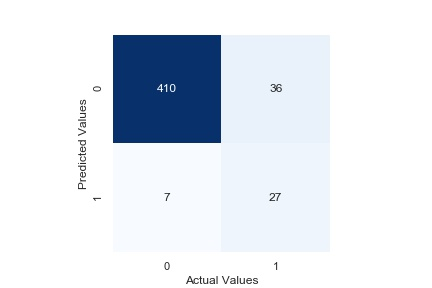
\includegraphics[scale=0.6]{img/twoclass_rf.jpg}
		\caption{Confusion matrix from Random Forest ran on testing data.}
		\label{confmatrf}
	\end{figure}

	The confusion matrix shows that the false negative and false positives are significantly lower than the true negatives and true positives. This shows that overall the Random Forest is performing quite well on the test data. The comparison between Random Forest and Support Vector Machine will be done later in this report. The next section will discuss Support Vector Machine (SVM) and the results for it.
	
	\section{Support Vector Machine (SVM)}
	Support Vector Machine (SVM) is a supervised machine learning algorithm that can be used for either regression or classification, in this case SVM will be used for classification. In this algorithm, each data point is plotted on a n-dimensional space and classification is performed by finding the hyperplane that differentiate between the classes well. In order to adjust the hyperplane, it uses the margin (distance between the hyperplane and the closest points to the hyperplane) to find the best hyperplane to classify the specific dataset. Similar to the implementation of Random Forest, SVM can be done with a built-in library in Python called \texttt{svm} in \texttt{sklearn}. To make a model, the hyperparameters does need to be adjusted and which method to use to determine the hyperplane. The methods include Radial Basis Functions (RBF), polynomial and linear. The metrics will be done using the same library as Random Forest.
	\subsection{Training \& Testing with RBFs}
	This is one of the 2 ways to determine a hyperplane that best fits the data. This way uses Radial Basis functions to determine the hyperplane. The algorithm tries to fit a function (described below) to the data and uses it as its model.
	\begin{align}
		K(x, x')=\text{exp}\left(-\frac{||x-x'||^2}{2\sigma^2}\right)
	\end{align}
	The results are presented below:\\\\\\\\\\
	\begin{table}[h]
		\centering
		\begin{tabular}{||c||c c c c||}
			\hline
			& \textbf{Precision} & \textbf{Recall} & \textbf{F1-Score} & \textbf{Support}\\
			\hline
			\hline
			0 & 1.00 & 0.56 & 0.71 & 63\\
			1 & 0.94 & 1.00 & 0.97 & 417\\
			\hline
			\hline
			Micro Avg & 0.94 & 0.94 & 0.94 & 480\\
			Macro Avg & 0.97 & 0.78 & 0.84 & 480\\
			Weighted Avg & 0.95 & 0.94 & 0.93 & 480\\
			\hline
		\end{tabular}
		\caption{Performance results from running model on testing data}
		\label{rbfsvmresults}
	\end{table}

	\noindent From the results presented in Table: \ref{rbfsvmresults} shows that the precision is at 95\%. This is a good sign that SVM with the kernel set to use RBFs is doing very well on the test data. Again, in order to see the number of true positives, false positives, true negatives and false negative, a confusion matrix is generated from the results.\\
	\begin{figure}[H]
		\centering
		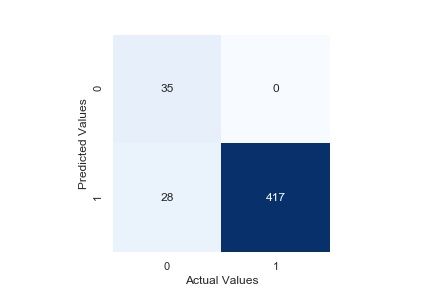
\includegraphics[scale=0.6]{img/twoclass_svmrbf.jpg}
		\caption{Confusion matrix from SVM with kernel set to use RBFs ran on testing data.}
		\label{svmrbfconfmat}
	\end{figure}
	From the confusion matrix (Figure: \ref{svmrbfconfmat}), the good wines are getting classified with no error while there is a error in classifying the poor wine. Judging from the dataset this may be due to the insufficient data for poor wine and the model isn't able to learn the best classifier. Can this result be improved by setting the kernel to use polynomials to determine the hyperplane?\footnote{works much better with polynomials!}
	\subsection{Training \& Testing with Polynomials}
	Here, the kernel is switched to use polynomials instead. This surprisingly works on the data with no problem. The preliminary results, without adjusting any of the other hyperparameters show a perfect performance on the test data. 
	\begin{table}[h]
		\centering
		\begin{tabular}{||c||c c c c||}
			\hline
			& \textbf{Precision} & \textbf{Recall} & \textbf{F1-Score} & \textbf{Support}\\
			\hline
			\hline
			0 & 1.00 & 1.00 & 1.00 & 63\\
			1 & 1.00 & 1.00 & 1.00 & 417\\
			\hline
			\hline
			Micro Avg & 1.00 & 1.00 & 1.00 & 480\\
			Macro Avg & 1.00 & 1.00 & 1.00 & 480\\
			Weighted Avg & 1.00 & 1.00 & 1.00 & 480\\
			\hline
		\end{tabular}
		\caption{Performance results from running model on testing data}
	\end{table}

	\noindent The confusion matrix showing a perfect classification as well!
	\begin{figure}[H]
		\centering
		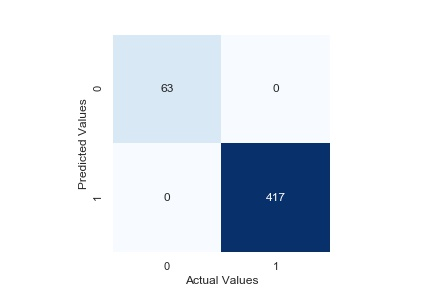
\includegraphics[scale=0.6]{img/twoclass_svmpoly.jpg}
		\caption{Confusion matrix from SVM with kernel set to use RBFs ran on testing data.}
	\end{figure}
	\section{Comparison of Random Forest v.s. SVM}
	From the preliminary results, SVM does classify this dataset better than Random Forests. Running SVM with the kernel set to use RBFs, it can perfectly classify all good wine compared to Random Forest where there is error in predicting both good and poor quality wine. Also with RBF SVM also performance marginally better in classifying poor quality wine as well. Looking deeper into these results may give a better picture on which machine learning algorithm performs better. By using Hoeffding's Inequality we can compute the 95\% confidence interval of the true risk for Random Forest and SVM.
	\subsection{Comparison Using Hoeffding's Inequality}
	For Random Forest, from the confusion matrix (Figure: \ref{confmatrf}), the loss is $\frac{36+7}{480}=\frac{43}{480}\approx 0.0896$. Setting $m=1599$, $\delta=0.05$ and $L_{S_{\text{test}}}=\frac{43}{480}$, the 95\% confidence interval is:
	\begin{align}
		\left[L_{S_{\text{test}}}-\sqrt{\frac{log\left(\frac{2}{\delta}\right)}{2m}},L_{S_{\text{test}}}+\sqrt{\frac{log\left(\frac{2}{\delta}\right)}{2m}}\right]=[0.0556,0.1235]
	\end{align}
	Next, for Support Vector Machine, similar to Random Forest, by observing the confusion matrix (Figure: \ref{svmrbfconfmat}), the loss is $\frac{28}{480}\approx 0.0583$. To compute the 95\% confidence interval, set $m=1599$, $\delta=0.05$ and $L_{S_{\text{test}}}=\frac{28}{480}$;
	\begin{align}
		\left[L_{S_{\text{test}}}-\sqrt{\frac{log\left(\frac{2}{\delta}\right)}{2m}},L_{S_{\text{test}}}+\sqrt{\frac{log\left(\frac{2}{\delta}\right)}{2m}}\right]=[0.0244,0.0922]
	\end{align}
	To get a clearer picture, here is a graph showing the 2 confidence intervals. We can see that RBF SVM does perform better than Random Forests as the upper bound on the true risk is lower compared to Random Forest. 
	\begin{figure}[H]
		\centering
		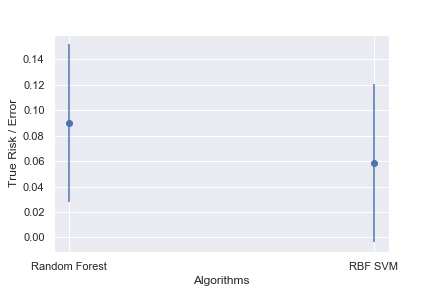
\includegraphics[scale=0.6]{img/binary_errorgraph.jpg}
		\caption{Plot of the 95\% confidence intervals for Random Forest and SVM}
	\end{figure}
\end{document}